\newpage

\section{ТЕСТИРОВАНИЕ}

\subsection{Описание входных и выходных данных}

При запуске программы читаются данные из файла, название которого вводится с клавиатуры. В процессе тестирования был создан файл <<Мировые рекорды>> (см. рисунок \ref{fig:data_tsv_github}, стр. \pageref{fig:data_tsv_github}).

\begin{figure}[!htp]
    \begin{center}
        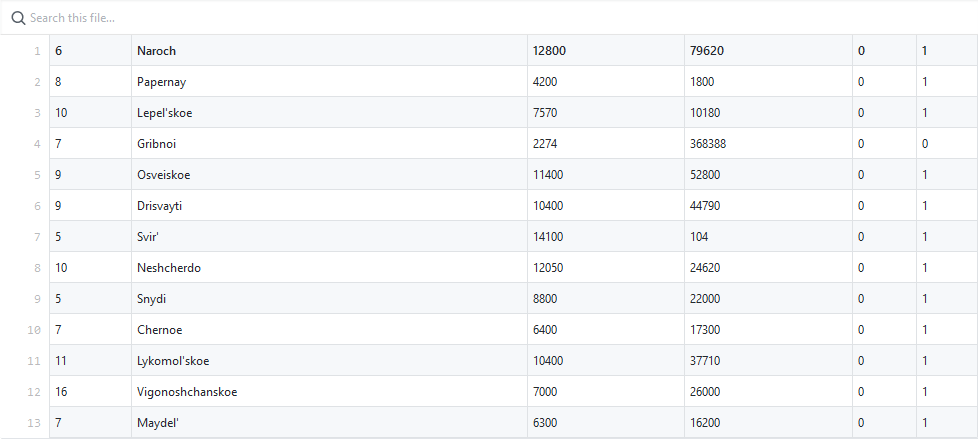
\includegraphics[width=14cm]{_input/tests/data-tsv-github.png}
    \end{center}
    \caption{Содержимое файла Мировые рекорды \label{fig:data_tsv_github}}
\end{figure}

\subsection{Результаты тестирования}

Среда тестирование – ПК, процессор Intel (R) Celeron (R) CPU N4060 с частотой 1.6 ГГц, ОЗУ 4 ГБ, тип системы: 64-разрядная OC Windows 10.

\hspace{0pt}\\



\textbf{Тест 1}: <<Ввод информации из текстового файла в список>>

\underline{Ожидаемый результат}: сформированный массив, содержащий данные считанные из текстового файла.

\underline{Описание}: тестирование правильности чтение информации из файла. Считывание происходит при выборе соответствующего пункта меню (см. рисунок \ref{fig:data_tsv}, стр. \pageref{fig:data_tsv}).

%\underline{Полученный результат}:

\begin{figure}[!hp]
    \begin{center}
        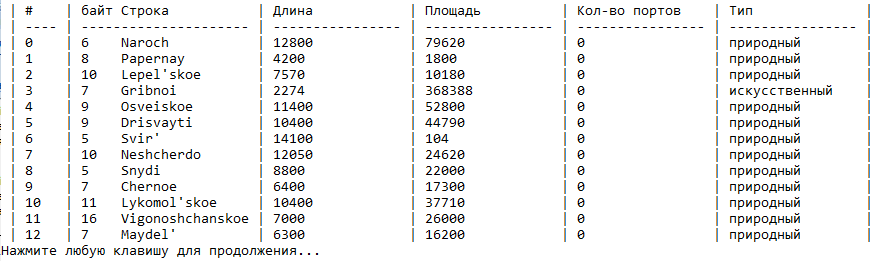
\includegraphics[width=16cm]{_input/tests/data-tsv.png}
    \end{center}
    \caption{Данные, считанные из файла\label{fig:data_tsv}}
\end{figure}

\underline{Вывод}: ввод информации из текстового файла работает корректно, массив, хранящий данные, считанные из файла, сформирован. Ожидаемый результат совпал с полученным. 

\hspace{0pt}\\



\textbf{Тест 2}: <<Добавление новых элементов в конец списка>>

\underline{Ожидаемый результат}: добавление новых записей в конец списка.

\underline{Описание}: тестирование правильности добавления новых элементов в конец списка. Добавление происходит при выборе соответствующего пункта меню. В исходный массив структурированных данных добавим записи Селява. Кривое, Ричи (см. рисунок \ref{fig:data_tsv_2}, стр. \pageref{fig:data_tsv_2}).

%\underline{Полученный результат}:

\begin{figure}[!hp]
    \begin{center}
        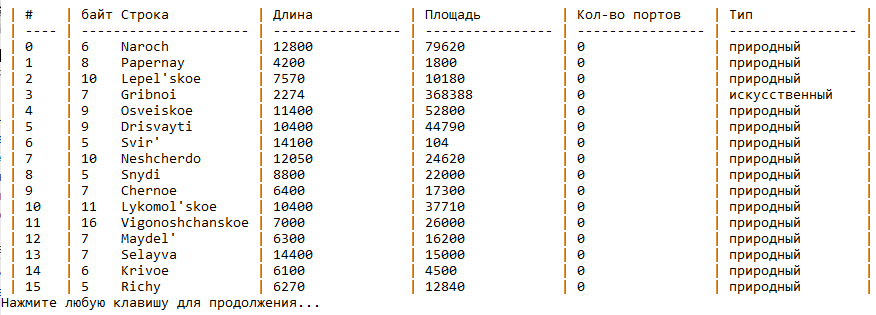
\includegraphics[width=16cm]{_input/tests/data-tsv-2.png}
    \end{center}
    \caption{Данные, находящиеся в массиве\label{fig:data_tsv_2}}
\end{figure}

\underline{Вывод}: добавление элементов в конец массива работает корректно. Ожидаемый результат совпал с полученным.

\hspace{0pt}\\



\textbf{Тест 3}: <<Корректировка полей выбранного элемента>>

\underline{Ожидаемый результат}: изменение данных, хранящихся в выбранном поле выбранной записи.

\underline{Описание}: тестирование правильности корректировки полей. Корректировка происходит после выбора соответствующего пункта меню, номера и поля изменяемой записи. Изменим кол-во портов в записи 3 (см. рисунок \ref{fig:data_tsv_3}, стр. \pageref{fig:data_tsv_3}).

%\underline{Полученный результат}:

\begin{figure}[!hp]
    \begin{center}
        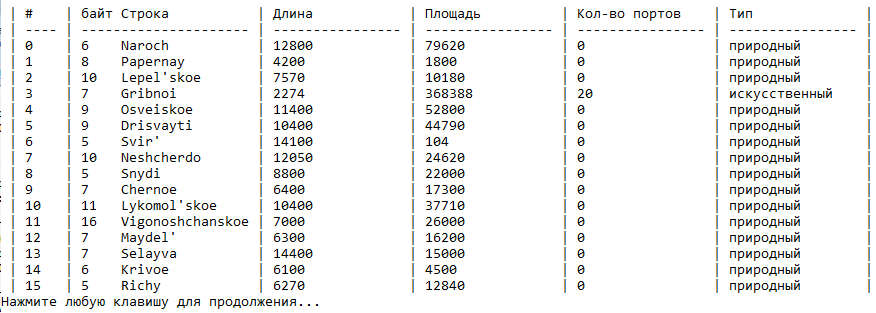
\includegraphics[width=16cm]{_input/tests/data-tsv-3.png}
    \end{center}
    \caption{Список после изменений\label{fig:data_tsv_3}}
\end{figure}

\underline{Вывод}: корректировка полей выбранного поля работает корректно. Ожидаемый результат совпал с полученным.

\hspace{0pt}\\



\textbf{Тест 4}: <<Удаление выбранного элемента>>

\underline{Ожидаемый результат}: удаление из списка выбранной записи.

\underline{Описание}: тестирование правильности удалениявыбранной записи. Удаление происходит после выбора соответствующего пункта меню и ввода автора удаляемой записи. В тестовом примере удалим записи Свири (6-ой) и Лукомольское (10-ое, которое станет 9-ое) (см. рисунок \ref{fig:data_tsv_4}, стр. \pageref{fig:data_tsv_4}).

%\underline{Полученный результат}:

\begin{figure}[!hp]
    \begin{center}
        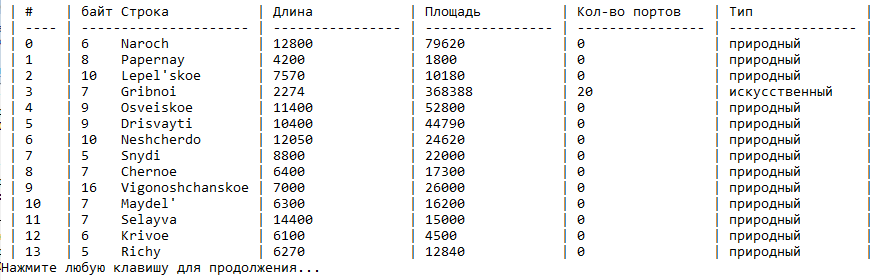
\includegraphics[width=16cm]{_input/tests/data-tsv-4.png}
    \end{center}
    \caption{Список после удаления\label{fig:data_tsv_4}}
\end{figure}

\underline{Вывод}: удаление выбранного элемента работает корректно. Ожидаемый результат совпал с полученным.

\hspace{0pt}\\



\textbf{Тест 5}: <<Сортировка записей по числовому Длина>>

\underline{Ожидаемый результат}: сортировка записей по длине по возрастанию.

\underline{Описание}: проверка корректности сортировки по числовому полю. Сортировка происходит после выбора соответствующего пункта меню (см. рисунок \ref{fig:data_tsv_5}, стр. \pageref{fig:data_tsv_5}).

%\underline{Полученный результат}:

\begin{figure}[!hp]
    \begin{center}
        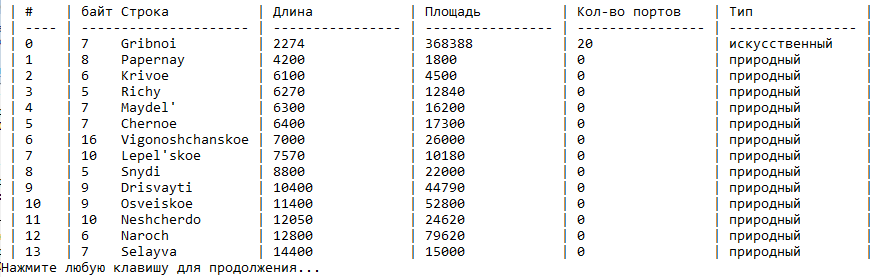
\includegraphics[width=16cm]{_input/tests/data-tsv-5.png}
    \end{center}
    \caption{Список после сортировки записей по длине\label{fig:data_tsv_5}}
\end{figure}

\underline{Вывод}: сортировка записей по числовому полю работает корректно. Ожидаемый результат совпал с полученным.